% --------------------------------------------------------------
% This is all preamble stuff that you don't have to worry about.
% Head down to where it says "Start here"
% --------------------------------------------------------------
 
\documentclass[12pt]{article}
 
\usepackage[margin=1in]{geometry} 
\usepackage{amsmath,amsthm,amssymb}
\usepackage{graphicx}
\usepackage{tikz}
\usetikzlibrary{arrows}
\newcommand{\N}{\mathbb{N}}
\newcommand{\Z}{\mathbb{Z}}
 
\newenvironment{theorem}[2][Theorem]{\begin{trivlist}
\item[\hskip \labelsep {\bfseries #1}\hskip \labelsep {\bfseries #2.}]}{\end{trivlist}}
\newenvironment{lemma}[2][Lemma]{\begin{trivlist}
\item[\hskip \labelsep {\bfseries #1}\hskip \labelsep {\bfseries #2.}]}{\end{trivlist}}
\newenvironment{exercise}[2][Exercise]{\begin{trivlist}
\item[\hskip \labelsep {\bfseries #1}\hskip \labelsep {\bfseries #2.}]}{\end{trivlist}}
\newenvironment{problem}[2][Problem]{\begin{trivlist}
\item[\hskip \labelsep {\bfseries #1}\hskip \labelsep {\bfseries #2.}]}{\end{trivlist}}
\newenvironment{question}[2][Question]{\begin{trivlist}
\item[\hskip \labelsep {\bfseries #1}\hskip \labelsep {\bfseries #2.}]}{\end{trivlist}}
\newenvironment{corollary}[2][Corollary]{\begin{trivlist}
\item[\hskip \labelsep {\bfseries #1}\hskip \labelsep {\bfseries #2.}]}{\end{trivlist}}
\newenvironment{solution}
  {\begin{proof}[Solution]\renewcommand{\qedsymbol}{}}
  {\end{proof}}

\usepackage{listings}
\usepackage{color}

\definecolor{mygreen}{rgb}{0,0.6,0}
\definecolor{mygray}{rgb}{0.5,0.5,0.5}
\definecolor{mymauve}{rgb}{0.58,0,0.82}

\lstset{ %
  backgroundcolor=\color{white},   % choose the background color; you must add \usepackage{color} or \usepackage{xcolor}
  basicstyle=\footnotesize,        % the size of the fonts that are used for the code
  breakatwhitespace=false,         % sets if automatic breaks should only happen at whitespace
  breaklines=true,                 % sets automatic line breaking
  captionpos=b,                    % sets the caption-position to bottom
  commentstyle=\color{mygreen},    % comment style
  deletekeywords={...},            % if you want to delete keywords from the given language
  escapeinside={\%*}{*)},          % if you want to add LaTeX within your code
  extendedchars=true,              % lets you use non-ASCII characters; for 8-bits encodings only, does not work with UTF-8
  frame=single,                    % adds a frame around the code
  keepspaces=true,                 % keeps spaces in text, useful for keeping indentation of code (possibly needs columns=flexible)
  keywordstyle=\color{blue},       % keyword style
  language=Python,                 % the language of the code
  morekeywords={*,...},            % if you want to add more keywords to the set
  numbers=left,                    % where to put the line-numbers; possible values are (none, left, right)
  numbersep=5pt,                   % how far the line-numbers are from the code
  numberstyle=\tiny\color{mygray}, % the style that is used for the line-numbers
  rulecolor=\color{black},         % if not set, the frame-color may be changed on line-breaks within not-black text (e.g. comments (green here))
  showspaces=false,                % show spaces everywhere adding particular underscores; it overrides 'showstringspaces'
  showstringspaces=false,          % underline spaces within strings only
  showtabs=false,                  % show tabs within strings adding particular underscores
  stepnumber=1,                    % the step between two line-numbers. If it's 1, each line will be numbered
  stringstyle=\color{mymauve},     % string literal style
  tabsize=2,                       % sets default tabsize to 2 spaces
  title=\lstname                   % show the filename of files included with \lstinputlisting; also try caption instead of title
}

\begin{document}


 
% --------------------------------------------------------------
%                         Start here
% --------------------------------------------------------------
 
\title{Homework 2}%replace X with the appropriate number
\author{Maksim Levental\\ %replace with your name
MAP 4102} %if necessary, replace with your course title
 
\maketitle
 
\begin{problem}{1} %You can use theorem, exercise, problem, or question here.  Modify x.yz to be whatever number you are proving
Using one-step analysis, compute $\rho_{AA}$ for an unbiased random walk on the following graph:

\begin{center}
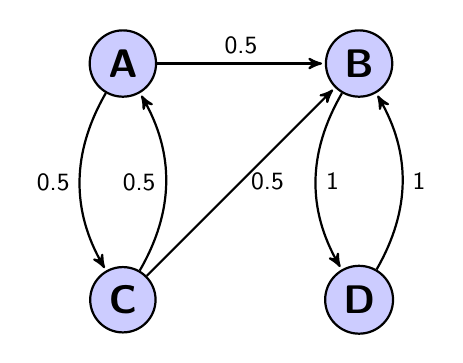
\begin{tikzpicture}[->,>=stealth',shorten >=1pt,auto,node distance=3cm,
  thick,main node/.style={circle,fill=blue!20,draw,font=\sffamily\Large\bfseries}]

  \node[main node] (1) {A};
  \node[main node] (2) [below of=1] {C};
  \node[main node] (3) [right of=1] {B};
  \node[main node] (4) [below of=3] {D};

  \path[every node/.style={font=\sffamily\small}]
    (1) edge node {0.5} (3)
        edge [bend right] node[left] {0.5} (2)
    (2) edge [bend right] node[left] {0.5} (1)
        edge node[right] {0.5} (3)
    (3) edge [bend right] node[right] {1} (4)
    (4) edge [bend right] node[right] {1} (3);
\end{tikzpicture}

\end{center}
\end{problem}
 
\begin{solution}
\begin{alignat*}{2}
\rho_{AA} &= \rho_{BA} \cdot p(A,B) + \rho_{CA} \cdot p(A,C) = \rho_{BA} \cdot \frac{1}{2} + \rho_{CA} \cdot \frac{1}{2} & \\
\rho_{CA} &= \rho_{AA'} \cdot p(C,A) + \rho_{BA} \cdot p(C,B) = 1 \cdot  \frac{1}{2} + \rho_{BA} \cdot \frac{1}{2} & \\
\rho_{BA} &= \rho_{DA} \cdot p(B,D) = 0 \cdot 1 = 0
\end{alignat*}
Note that $\rho_{AA}$ and $\rho_{AA'}$ are different; $\rho_{AA}$ is the probability of hitting $A$ for some time $n\geq 1$ and $\rho_{AA'}$ is the probability of hitting $A$ for sometime $n \geq i$ given that $X_i = A$. Hence
\begin{alignat*}{2}
\rho_{CA} &= 1 \cdot \frac{1}{2} + 0 \cdot \frac{1}{2} = \frac{1}{2} \\
\rho_{AA} &= 0 \cdot \frac{1}{2} + \frac{1}{2} \cdot \frac{1}{2} = \frac{1}{4} \\
\end{alignat*}



\end{solution}

\ \\ \\

\begin{problem}{2} %You can use theorem, exercise, problem, or question here.  Modify x.yz to be whatever number you are proving
Compute $\rho_{00}$ for an unbiased random walk on the following graph


\begin{center}
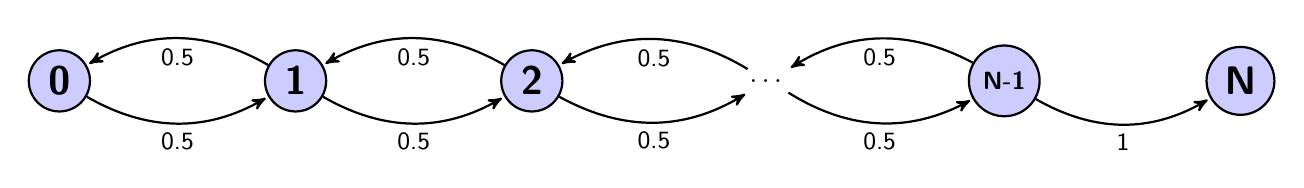
\begin{tikzpicture}[->,>=stealth',shorten >=1pt,auto,node distance=3cm,
  thick,main node/.style={circle,fill=blue!20,draw,font=\sffamily\Large\bfseries}]

  \node[main node] (1) {0};
  \node[main node] (2) [right of=1] {1};
  \node[main node] (3) [right of=2] {2};
  \node[draw = none] (4) [right of=3] {\dots};
  \node[main node] (5) [right of=4] {\small{N-1}};
  \node[main node] (6) [right of=5] {N};

  \path[every node/.style={font=\sffamily\small}]
    (1) edge [bend right] node[below] {0.5} (2)
    (2) edge [bend right] node[below] {0.5} (1)
        edge [bend right] node[below] {0.5} (3)
    (3) edge [bend right] node[below] {0.5} (2)
        edge [bend right] node[below] {0.5} (4)
    (4) edge [bend right] node[below] {0.5} (3)
        edge [bend right] node[below] {0.5} (5)
    (5) edge [bend right] node[below] {0.5} (4)
        edge [bend right] node[below] {1} (6);
\end{tikzpicture}

\end{center}

\end{problem}
 
\begin{solution} 
We claim that 
$$\rho_{00}=1-\frac{1}{M-1}$$ 
where $M$ is the number of nodes, or $1 - \frac{1}{N}$ if we abide by the numbering scheme above.
\end{solution}
\begin{proof}
For arbitrary state $x$, with the exception of $\rho_{00}$ and $\rho_{N0}$,
$$\rho_{x0} = \rho_{(x-1)0}\cdot \frac{1}{2} + \rho_{(x+1)0}\cdot\frac{1}{2}.$$
Summing $\rho_{x0}$ and $\rho_{(x+1)0}$ we get
$$ \rho_{x0} + \rho_{(x+1)0} = \rho_{(x-1)0}\cdot \frac{1}{2} + \rho_{(x+1)0}\cdot\frac{1}{2} + \rho_{(x)0}\cdot \frac{1}{2} + \rho_{(x+2)0}\cdot\frac{1}{2}. $$
Rearranging, combining like terms, and cancelling the common factor of $\frac{1}{2}$ yields
$$ \rho_{x0} - \rho_{(x-1)0} = \rho_{(x+2)0} - \rho_{(x+1)0}\ . $$
Hence 
$$ \rho_{20} - \rho_{10} = \rho_{40}\ - \rho_{30} = \ldots = \rho_{N0} - \rho_{(N-1)0}. $$
But $\rho_{N0} = 0$, because it's an absorbing state. Hence
$$ \rho_{20} - \rho_{10} = \rho_{40}\ - \rho_{30} = \ldots = - \rho_{(N-1)0} $$
$$ \rho_{10} - \rho_{20} = \rho_{30} - \rho_{40}  = \ldots =  \rho_{(N-1)0}. $$
 This shows that $\rho_{x0}$ decreases to zero in increments of $\rho_{(N-1)0}$. Let $ \rho_{(N-1)0} = K$ for some yet to be determined constant $K$ and $M$ be the number of nodes. Hence $\rho_{10} = (M-2) \cdot K$ ($M-2$ incremental ``subtractions'' occur state $1$ and state $M$). But then
$$\rho_{10} = (M-2) \cdot K =  \rho_{00'} \cdot \frac{1}{2} + \rho_{20} \cdot \frac{1}{2} = 1 \cdot \frac{1}{2} + \rho_{20} \cdot \frac{1}{2} $$
where $\rho_{00'} = 1$ because $\rho_{00'}$ is the probability of hitting $0$ for sometime $n \geq i$ given that $X_i = 0$. Since similarly $\rho_{20} = (M-3) \cdot K$ it follows that
$$ (M-2) \cdot K =  1 \cdot \frac{1}{2} +  \frac{1}{2} (M-3) \cdot K $$
$$ K = \frac{1}{M-1} $$
Hence $\rho_{10} = (M-2) \frac{1}{M-1} = 1 - \frac{1}{M-1}$ and 
$$\rho_{00} = \rho_{10} = 1 - \frac{1}{M-1} =  1 - \frac{1}{(N+1)-1} = 1 - \frac{1}{N}$$.
\end{proof}

\noindent For the instances where $M = {2,3,4}$ (corresponding to $N = {1,2,3}$) $\rho_{00}=0,\frac{1}{2},\frac{2}{3}$. In the limit as $N \rightarrow \infty$ the probability of returning is clearly $1$.
\ \\

Numerical computation confirms this:
\ \\

\noindent \texttt{randomwalk.py}
\begin{lstlisting}[language=Python]
import sys
from random import choice

direction = [1,-1]
returns = 0.
k = int(sys.argv[2])
n = int(sys.argv[1])
for i in range(k):
	step = 1
	while step != 0 and step !=n:
		step += choice(direction)
	if(step == 0):
		returns += 1
	
print returns/k
\end{lstlisting}

\begin{lstlisting}[language=bash]
  $ python randomwalk.py 1 10000
  $ 0.0
  $ python randomwalk.py 2 10000
  $ 0.4986
  $ python randomwalk.py 3 10000
  $ 0.6733
  $ python randomwalk.py 10 10000
  $ 0.9017
\end{lstlisting}

% --------------------------------------------------------------
%     You don't have to mess with anything below this line.
% --------------------------------------------------------------
 
\end{document}
\begin{align*}
\sum_{i=1}^{k+1}i & = \left(\sum_{i=1}^{k}i\right) +(k+1)\\ 
& = \frac{k(k+1)}{2}+k+1 & (\text{by inductive hypothesis})\\
& = \frac{k(k+1)+2(k+1)}{2}\\
& = \frac{(k+1)(k+2)}{2}\\
& = \frac{(k+1)((k+1)+1)}{2}.
\end{align*}
